\setlength\abovedisplayskip{2.5pt}

For relevant nuclear forensics predictions, both classification and regression
algorithms must be used.  For example, one may want to predict the reactor type
label given some measurement-based features of \gls{SNF} of an unknown source.
This would require a classification algorithm. Or perhaps the input fuel
composition is relevant to an investigation on weapons intent, so a regression
algorithm would be used. 

\subsubsection{Nearest Neighbor Methods}

Nearest neighbor regression is a unique algorithm in that it is instance-based;
it does not actually generalize, but tracks the observations in the training
set.  The main metric for this algorithm is distance (or dissimilarity) between
the test sample and the closest training sample(s) in the vicinity.  During
prediction, the algorithm will calculate a value based on the instance that is
closest to the current test sample. Thus, there is not any learning, but
instead a direct comparison between an unknown sample and the space that the
training set populates. The predictions from nearest neighbors can be quite
accurate, but are highly unstable to peturbations \cite{elements_stats}.

\begin{figure}[!htb]
  \centering
  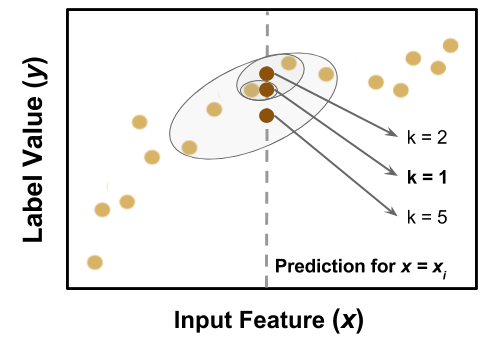
\includegraphics[width=0.8\linewidth]{./chapters/litrev/nn-fig.png}
  \caption{Schematic of \textit{k}-nearest neighbors regression, showing how 
           changing \textit{k} alters the predicted label value $y$.}
  \label{fig:nn}
\end{figure}

An extension of nearest neighbor is \textit{k}-nearest neighbor regression.
The closest \textit{k} neighbors are averaged for an estimate of the unknown
sample, as shown in Equation \ref{eq:knn}.  Figure \ref{fig:nn} provides a
pictoral explanation of how this is done for a prediction of a single feature.
For \textit{k}-neighbors, this algorithm predicts a value, $Y$, from the input
features, $\boldsymbol{X}$, in the neighborhood, $N_k (\boldsymbol{X})$
\cite{elements_stats}. 
\begin{equation}
  Y(\boldsymbol{X}) = \frac{1}{k} \sum_{x_i \in N_k(\boldsymbol{X})} y_i
  \label{eq:knn}
\end{equation}

There are two tuneable parameters in this algorithm: the distance metric and
the value of \textit{k}.  The population of the neighborhood, \textit{k},
affects the number of points being averaged together for a prediction.  The
metrics for distance can be the Manhattan distance, Euclidian distance, 
\todo[inline]{finish me}

\subsubsection{Decision Trees}
To write: a section on decision trees

\subsubsection{Maximum Log-Likelihood Calculations}
To write: a section on \gls{MLL} calcs.

